In rare occasioni vediamo \textit{violazioni} di leggi di conservazione, che sono valide solo per interazione forte ed elettromagnetica. Queste sono note come \textit{interazioni deboli} (w.i.) a causa della loro piccola costante di accoppiamento. L'interazione debole avviene in quasi tutti i processi ma il loro effetto è trascurabile, eccetto nei casi in cui tutto il resto è proibito (e.g. decadimenti che violano la stranezza, charm,\dots). A causa della interazione forte, la materia \textit{stabile} è formata solo da $u,d,e^-$. Gli altri quark e leptoni carichi sono instabili e decadono debolmente. Dunque nonostante la loro "debolezza" (piccolo range di interazione $10^{-3}$ fm e piccole sezioni d'urto $10^{-47}$ m$^2$), l'interazione forte assume un ruolo fondamentale nel determinare il nostro mondo.\\
\textit{Tutte} le particelle elementari, eccetto gluoni e fotoni (mediatori dell'interazione), vedono l'interazione debole: i quark ed i leptoni carihi interagiscono debolmente, i neutrini interagiscono \textit{solo} debolmente. Per questo motivo la nostra conoscenza dell'interazione debole, almeno fino agli anni 70, si ottenne solo da decadimenti di particelle (e.g. $\pi^+$ e $\mu^+$ che decadono) e da fasci di neutrini.
\subsubsection{Piccolo ripassino}
Rivediamo i tempi di vita media di alcuni decadimenti:
\begin{alignat*}{3}
    &\Delta^{++} \to p\pi &&\sim 10^{-23}s &&\textnormal{int. forte} \\
    &\Sigma^0\to\Lambda\gamma &&\sim6\cdot10^{-20}s \textnormal{ }&& \textnormal{int. e.m. (c'è un }\gamma) \\
    & \pi^0\to\gamma \gamma &&\sim 10^{-16}s && \textnormal{int. e.m. (ci sono due }\gamma)
\end{alignat*}
\begin{align*}
    & \begin{aligned}
       & \Sigma\to n\pi &&\sim10^{-10}s \\
       & \pi^-\to\mu\nu_\mu&&\sim10^{-8}s \\
       & \mu^-\to e^-\bar\nu_e\nu_\mu&&\sim10^{-6}s \\
       & n\to pe^-\bar\nu_e&&\sim15\textnormal{ min}
    \end{aligned}
     \left.\vphantom{\begin{matrix}
    \text{Equazione 7}\\
    \text{Equazione 8}\\
    \text{Equazione 9}\\
    \text{Equazione 10}
    \end{matrix}}\right\} \text{int. debole}
    \end{align*}
\begin{itemize}
    \item Dobbiamo spiegare l'enorme intervallo di tempi di vita media che va da $10^{-12}$ s a 15 min.
    \item L'interazione debole è anche caraterizzata da sezioni d'urto estremamente piccole \\
    ($\sim10^{-39}cm^2=1$ fb)
    \begin{alignat*}{3}
    &\sigma(\nu_\mu+N\to N+\pi+\mu)&&=10^{-38}\textnormal{cm}^2(10\,\textnormal{fb}) &&\textnormal{ ad 1 GeV}\\
    &\sigma(\pi+N\to N+\pi)&&=10^{-26}\textnormal{cm}^2(10\,\textnormal{mb}) &&\textnormal{ ad 1 GeV}
    \end{alignat*}
    \item L'interazione debole viola molte leggi di conservazione: parità, coniugazione di carica, stranezza, etc.
    \item Come già detto, a causa della loro debolezza, l'interazione debole può essere osservata nella materia ordinaria solo nel decadimento $\beta$, perché non da origine ad alcun stato legato. Tuttavia, sono la base del funzionamento delle stelle che senza di essa non esisterebbe:
    \begin{equation*}
    p+p\to d+e^++\nu_e
    \end{equation*}
\end{itemize}
\subsubsection{Corrente carica e corrente neutra}
Nel modello standard, l'interazioni deboli sono classificate in due tipologie, in base alla carica del mediatore:
\begin{itemize}
    \item \textbf{Correnti cariche (CC)}, scambio di $W^\pm$: nei processi CC, la carica dei quark e leptoni cambia di $\pm1$; allo stesso tempo c'è una variazione della loro identità, cioè del flavour, secondo la teoria di Cabibbo.
    \begin{figure}[H]
        \centering
        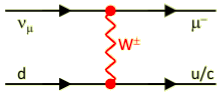
\includegraphics[width=0.5\textwidth]{immagini/fig_cc_process.png}
        \caption{Processo di corrente carica. Un $d$ emette $W^-$ e diventa $u$.}
        %\label{fig:cc_process}
    \end{figure}
    \item \textbf{Correnti neutre (NC)}, scambio di $Z$: in questo caso i quark ed i leptoni restano invariati (non c'è FCNC Flavour-Changing Neutral Current). Fino al 1973 nessun processo NC fu osservato, anche se un esempio evidente lo abbiamo ossia il $\gamma$ della interazione elettromagnetica non porta alcuna carica.
    \item Negli anni 60 Glashow, Salam e Weinberg (e molti altri teorici) svilupparono una teoria, oggi parte del Modello Standard, che unifica la interazione debole (sia CC che NC) e l'elettromagnetismo.
    \item Il Modello Standard fu ideato \textit{prima} della scoperta di NC e del suo portatore (bosone $Z$), predetto dal Modello Standard negli anni 60 e direttamente osservato al CERN nel 1983.
\end{itemize}
\subsubsection{Classificazione}
\begin{minipage}{0.6\textwidth}
    \begin{figure}[H]
        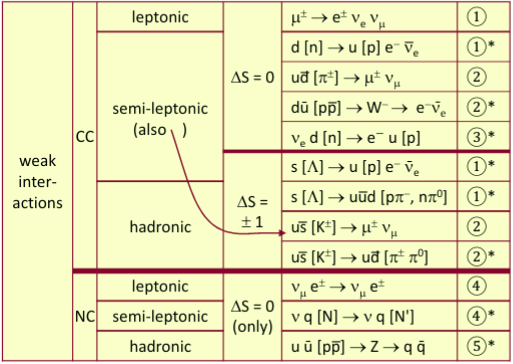
\includegraphics[width=\textwidth]{immagini/fig_table_weak_int.png}
        %\caption{Tabella delle interazioni deboli.}
        %\label{fig:table_weak_int}
    \end{figure}
    Nell'ultima colonna l'asterisco indica che l'adrone interagente, mostrato tra le parentesi quadre, è composto. Nei diagrammi ci sono solo i quark interagenti. Gli altri partoni spettatori non partecipano alla interazione.
\end{minipage}
\begin{minipage}{0.30\textwidth}
\begin{figure}[H]
    \centering
    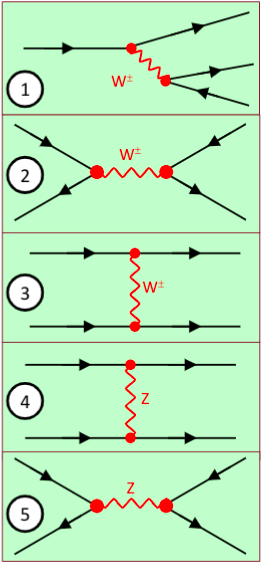
\includegraphics[width=\textwidth]{immagini/fig_xchange_bosons.png}
    %\caption{Scambio di bosoni nell'interazione debole.}
    %\label{fig:xchange_bosons}
\end{figure}
\end{minipage}
\subsection{Correnti cariche}
Abbiamo detto che una caratteristica dell'interazione debole è il grande range di possibili vite medie, rispetto a quello di interazione forte ed elettromagnetica che è ristretto.
\begin{table}[h!]
    \centering
    \begin{tabular}{|c|c|l|}
        \hline
        \textbf{Processo} & \textbf{Vita media (s)} & \textbf{Commento} \\
        \hline
        $\bar{\nu}_e p \to n e^+$ & infinita & I neutrini interagiscono solo debolmente (non decadono) \\
        \hline
        $n \to p e^- \bar{\nu}_e$ & $\mathcal{O}(10^3)$ & Lunga vita a causa della piccola differenza in massa p-n \\
        \hline
        $\pi^+ \to \mu^+ \nu_\mu$ & $\mathcal{O}(10^{-8})$ & I $\pi^\pm$ sono gli adroni più leggeri, dunque decadono in leptoni\\
        \hline
        $\Lambda \to p \pi^-$ & $\mathcal{O}(10^{-10})$ & Il decadimento di $\Lambda$ viola la conservazione di stranezza \\
        \hline
    \end{tabular}
    %\caption{Summary of particle decay processes.}
\end{table}
\begin{figure}[H]
    \centering
    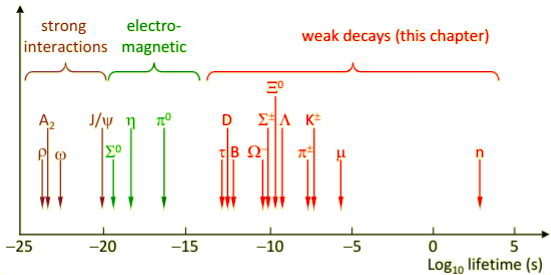
\includegraphics[width=0.6\textwidth]{immagini/fig_decay_sketch.png}
    \caption{I decadimenti deboli più interessanti sono di solito quelli dei mesoni pesanti e.g. $K^0$ e $ B^0$.}
    %\label{fig:decay_sketch}
\end{figure}
\subsubsection{Teoria di Fermi}
\begin{itemize}
    \item La teoria moderna delle interazioni con corrente carica (una parte del Modello Standard) è il il successore della teoria di Fermi del decadimento $\beta$. 
    \item La teoria descrive l'interazione come puntuale e proporzionale alla costante d'accoppiamento $G_F$. Tuttavia, c'era un problema intrinseco in essa, ossia che non è rinormalizzabile, cioè che le sezioni d'urto divergono ad alte energie.
    \item Il Modello Standard rispetto alla teoria di Fermi va oltre l'interazione puntuale, introducendo un mediatore pesante, chiamato $W^\pm$.
    \item Il Modello Standard è matematicamente consistente, cioè è rinormalizzabile.
    \item Ma più importante è che il Modello Standard riproduce i dati sperimentali con precisione mai vista prima.
\end{itemize}
\begin{figure}[H]
    \centering
    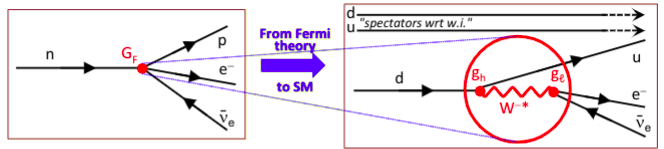
\includegraphics[width=0.6\textwidth]{immagini/fig_fermi_to_ms.png}
    \caption{Transizione dalla teoria di Fermi al Modello Standard con i mediatori.}
    %\label{fig:fermi_to_ms}
\end{figure}
Perché il decadimento forte $n\to \pi^-p$, simile a $\Delta^0\to p\pi^-$, è proibito?
\begin{figure}[H]
    \centering
    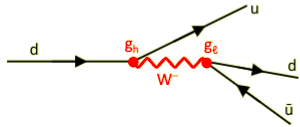
\includegraphics[width=0.6\textwidth]{immagini/fig_n_p_pi.png}
    %\caption{Il decadimento forte $n\to \pi^-pp$ è proibito a causa della conservazione del numero barionico.}
    %\label{fig:n_p_pi}
\end{figure}
Dinamicamente è possibile, tuttavia, la differenza in massa tra neutroni e protoni è di 1.3 MeV, dunque l'unica possibile coppia fermione/antifermione con carica -1 e numero leptonico/barionico nullo è chiaramente $e^-\bar \nu_e$, perché $m(e^-)+m(\bar\nu_e)\approx m(e^-)\approx0.5$ MeV. Invece non produco pioni perché la massa del pione è 140 MeV, superiore agli 1.3 MeV a disposizione. 
\subsubsection{Costante di accoppiamento}
Ad ogni vertice di interazione nel diagramma di Feynman corrisponde una costante di accoppiamento.
\begin{itemize}
    \item Nel caso elettromagnetico la costante di accoppiamento $\alpha\propto e^2$, da cui anche la ampiezza. Invece il rate (o la sezione d'urto) proporzionale al quadrato dunque $\sigma\propto\alpha^2\propto e^4$ 
    \item Nel caso di interazioni deboli la costante di accoppiamento è $G_F$ ed è proporzionale a $g^2$, che assume il ruolo di carica della interazione debole (analoga ad $e$). Dunque l'ampiezza sarà $\propto g^2$ e $\sigma\propto g^4$.s
    \item Al contrario di $\alpha$, la $G_F$ non è adimensionata: ha le dimensioni di $E^{-2}$.
\end{itemize}
\subsection{Decadimento \texorpdfstring{$\beta$}{β}}
\[
\begin{aligned}
&n \to p + e^- + \bar{\nu}_e &\implies (A, Z) \to (A, Z+1) + e^- + \bar{\nu}_e \\
&p \to n + e^+ + \nu_e &\implies (A, Z) \to (A, Z-1) + e^+ + \nu_e \\
&p + e^- \to n + \nu_e &\implies (A, Z) + e^- \to (A, Z-1) + \nu_e
\end{aligned}
\]
\begin{itemize}
    \item L'esistenza del decadimento $\beta$ si ebbe nel 1934 con Curie.
    \item Nel 1919 Chadwick scoprì che l'elettrone proveniente dal $\beta$-decay ha uno spettro continuo.
\end{itemize}
\begin{minipage}{0.6\textwidth}
    \begin{figure}[H]
        \centering
        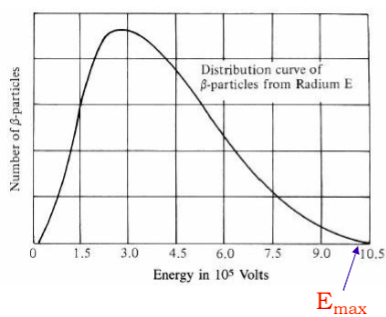
\includegraphics[width=\textwidth]{immagini/fig_beta_decay.png}
        %\caption{Spettro continuo del decadimento $\beta$.}
        %\label{fig:beta_decay}
    \end{figure}
\end{minipage}
\begin{minipage}{0.39\textwidth}
    \begin{itemize}
        \item Il massimo in energia nello spettro corrisponde abbastanza bene al $Q$-value della reazione, mentre per il resto dello spettro c'è una violazione della conservazione di energia.
        \item Inoltre c'è una violazione della conservazione dell'impulso e del momento angolare (senza l'introduzione del neutrino).
    \end{itemize}
\end{minipage}
\subsubsection{Il neutrino}
Per ristabilire le varie leggi di conservazione, Pauli nel 1930 ipotizzò l'esistenza del neutrino. 
\begin{itemize}
    \item La teoria di Fermi del decadimento $\beta$ fu fatta nel 1934
    \item La scoperta del neutrino avvenne nel 1958 da parte di Reines e Cowan.
    \item Abbiamo tre tipi di neutrini. Recentemente si sono scoperte le oscillazioni in flavour del neutrino che implicano che la loro massa è non nulla, sebbene sia molto piccola e ancora non misurata.
    \item Quello di Pauli era un tentativo disperato di spiegare lo spettro continuo delle emissioni $\beta$. Pauli lo chiamò "neutrone", ma poi questo nome fu dato alla particella scoperta da Chadwick nel 1932 un anno dopo. Come tutti a quell'epoca, Pauli credette che se un nucleo radioattivo emette particelle, queste devono esistere nel nucleo prima dell'emissione.
\end{itemize}
\subsubsection{Approccio di Fermi per la sua teoria}
Per formulare la sua teoria, Fermi prese come modello quello che già si sapeva ossia la QED (interazione elettromagnetica). \\
Consideriamo lo scattering elettrone-protone:\\
\begin{minipage}{0.3\textwidth}
    \begin{figure}[H]
        \centering
        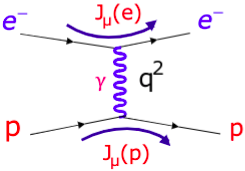
\includegraphics[width=\textwidth]{immagini/fig_electron_proton_scattering.png}
        %\caption{Scattering elettrone-protone.}
        %\label{fig:electron_proton_scattering}
    \end{figure}
\end{minipage}
\begin{minipage}{0.65\textwidth}
    Dal diagramma di Feynman, l'elemento di matrice sarà
    \begin{equation*}
    M\_{fi}\approx-\frac{1}{q^2}J_\mu(e)J^\mu(p)
    \end{equation*} 
    dove $q$ è il propagatore. In generale si scrive 
    \begin{equation*}
    M\_{fi}\approx\qty(\bar u_e\sqrt\alpha\gamma^\mu u_e)\frac{g_{\mu\nu}}{q^2}\qty(\bar u_p\sqrt\alpha\gamma^\nu u_p)
    \end{equation*} 
\end{minipage}
Dunque a partire da ciò, Fermi ipotizzo che l'interazione debole fosse puntiforme: $n+\nu\to p+e^-$\\
\begin{minipage}{0.3\textwidth}
    \begin{figure}[H]
        \centering
        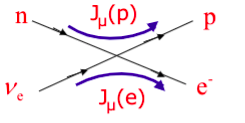
\includegraphics[width=\textwidth]{immagini/fig_diag_weak_int_fermi.png}
        %\caption{Interazione debole puntiforme.}
        %\label{fig:weak_interaction}
    \end{figure}
\end{minipage}
\begin{minipage}{0.65\textwidth}
    Dunque stavolta non c'è propagatore!\\
    \begin{equation*}
    M\_{fi}\approx G\qty(\bar u_p\gamma^\mu u_n)\qty(\bar{u}_e\gamma_\mu u_\nu)
    \end{equation*}
    ed è una interazione vettore-vettore perché "$\gamma^\mu$ è di dimensione 4". \\
    La costante $G$ è nota come costante di Fermi ed è legata al quadrato della \textit{carica debole}.
\end{minipage}
Si ha interazione tra due correnti cariche: si possono avere correnti adroniche e correnti leptoniche. Al solito $u_p$ distrugge la particella $p$ mentre $\bar{u}_p$ crea la particella $p$. Ad alte energie la teoria di Fermi non funziona più.
\subsubsection{Decadimento nucleare $\beta$}
La probabilità di transizione su unità di tempo si può ricavare con la regola d'oro di Fermi:
\begin{equation*}
W=\frac{2\pi}{\hbar}G^2\abs{M}^2\dv{N}{E_0}\qq{}\dv{N}{E_0}:\textnormal{ fattore dello spazio delle fasi}
\end{equation*}
Il termine $\abs{M}^2$ è il quadrato dell'elemento di matrice. Si determina integrando su tutti gli angoli delle particelle finali, sommando su tutti i possibili stati di spin finali e mediando sugli stati di spin iniziali. Il valore risultante è una costante dell'ordine di uno.\\
Con $E_0$ indichiamo l'energia disponibile nello stato finale, uguale al $Q$ della reazione. Lo spread energetico $\dd{E_0}$ è presente perché l'energia dello stato iniziale è indeterminata dal fatto che ha vita media finita (principio di indeterminazione).\\
Nel decadimento $\beta$ normalmente $E_0\approx1$ MeV. L'energia cinetica del protone è dell'ordine di $10^{-3}$ MeV e può essere trascurata. Il protone serve solo ad assicurarci che ci sia la conservzione dell'impulso. Dunque possiamo considerare suppore che l'energia finale sia suddivisa tra neutrino ed elettrone $E_0=E_e+q_\nu$.
\subsubsection{Spazio delle fasi}
\begin{itemize}
    \item Il numero di stati disponibili per un elettrone di impulso tra $p$ e $p+\dd{p}$ confinato nel volume $V$ entro un angolo solido $\dd{\Omega}$ è:
    \begin{equation*}
    \dd{N}=\frac{V\Omega}{\qty(2\pi)^3\hbar^3}p^2\dd{p}
    \end{equation*}
    \item Normalizziamo la funzione d'onda con $V=1$, e sommiamo su tutto l'angolo solido ignorando lo spin. Otteniamo
    \begin{equation*}
    \dd{N_e}=\frac{4\pi p^2\dd{p}}{\qty(2\pi)^3\hbar^3}\qq{}\dd{N_\nu}=\frac{4\pi q_\nu^2\dd{q_\nu}}{\qty(2\pi)^3\hbar^3} 
    \end{equation*}
    \item I due fattori di spazio delle fasi sono indipendenti in quanto non c'è correlazione tra $q$ e $p$, visto che nel decadimento a tre corpi il protone assorbirà la differenza di impulso. Il protone ha impulso fissato, dato da $q$ e $p$, così che il protone non ha fattore di spazio delle fasi.
    \item Il numero di stati finale è 
    \begin{equation*}
    \dd{N}=\dd{N_e}\dd{N_\nu}=\frac{\qty(4\pi)^2}{\qty(2\pi)^6\hbar^6}p^2q_\nu^2\dd{p}\dd{q_\nu}
    \end{equation*}
    \item Per un dato valore di energia dell'elettrone $E$, l'energia del neutrino $E_\nu$ p fissata, così come il suo impulso:
    \begin{equation*}
    q_\nu=E_\nu=E_0-E\implies\dd{q_\nu}=\dd{E_0}\implies\dv{N}{E_0}=\dv{N}{q_\nu}=\frac{1}{4\pi^4\hbar^6}p^2(E_0-E)^2\dd{p}
    \end{equation*}
    \item Una volta che abbiamo integrato la probabilità di transizione $W$ su tutto l'angolo solido, $\abs{M}^2$ è uguale ad una costante, dunque lo spettro energetico dell'elettrone dipende soltanto dal fattore di spazio delle fasi:
    \begin{equation*}
    N(p)\dd{p}\propto p^2(E_0-E)^2\dd{p}
    \end{equation*}
\end{itemize}
\subsubsection{Kurie plot}
\begin{itemize}
    \item Se facciamo il grafico di $\qty(\frac{N(p)}{p^2})^{\frac{1}{2}}$ in funzione dell'energia dell'elettrone, otteniamo una retta che interseca l'asse $x$ in $E=E_0$. Questo plot fu sviluppato da Kurie.
    \item Sperimentalmente dobbiamo includere un fattore correttivo $F(Z,p)$ per tenere conto dell'interazione coulombiana tra elettrone e nuclei.
    \item Se il neutrino avesse massa, i suoi effetti modificherebbero la distribuzione:
    \begin{equation*}
    N(p)\dd{p}\propto p^2(E-E_0)^2\sqrt{1-\qty(\frac{m_\nu}{E_0-E})^2}\dd{p}
    \end{equation*}
    \item Il plot di Kurie è modificato in modo che la curva intersechi l'asse $x$ in $E=E_0-m_\nu$. Questo è un tentativo di misurare la massa del neutrino elettronico... Sfortunatamente in questa regione ci sono pochi eventi per difficoltà sperimentali/tecniche. Al momento abbiamo solo un limite superiore
    \begin{equation*}
    m_\nu\leq2.2 \eV
    \end{equation*}
\end{itemize}
\subsubsection{La regola di Sargent}
\begin{itemize}
    \item Il rate totale di decadimento si ottiene integrando lo spettro $N(p)\dd{p}$. Si può fare analiticamente, tuttavia considerando l'elettrone relativisticamente (cioè quasi sempre) possiamo approssimare $p\approx E$ ed ottenere una formula semplice:
    \begin{equation*}
    N\propto\int_{0}^{E_0}E^2(E_0-E)^2\dd{E}\propto E_0^5
    \end{equation*}
    \item Il rate di decadimento è proporzionale alla quinta potenza dell'energia disponibile nel processo. Questa è la regola di Sargent. 
    \item Considerando tutti i fattori numerici nel processo, otteniamo 
    \begin{equation*}
        W=\frac{G^2\abs{M}^2E_0^5}{60\pi^3(\hbar c)^6\hbar}\qq{Per }E_0\gg m_e
    \end{equation*}
    \item La costante di Fermi $G$ si può ricavare da misure di tempo di vita media di decadimenti $\beta$ (e qualche speculazione teorica, vedi angoli di Cabibbo) o in modo più preciso dalla vita media del $\mu$.
    \item Dalla PDG otteniamo $\frac{G}{(\hbar c)^3}=1.16637(1)\cdot10^{-5}\textnormal{ GeV}^{-2}$
    \item Sostituendo valori numerici otteniamo $\frac{1}{\tau}=W=\frac{1.11}{10^4}\abs{M}^2E_0^5s^{-1}$\qq{($E_0$ in MeV)}
    \item Per esempio se $E_0\approx100$ MeV come nel decadimento del muone e $\abs{M}^2=1$, otteniamo
    \begin{equation*}
    \tau_\mu=\frac{1}{W}\approx10^{-6}s\qq{$\tau_\mu=2.2\mu$s}
    \end{equation*}
    \item La dipendenza da $E_0^5$ spiega il grande range di tempi di vita media dei decadimenti deboli.
\end{itemize}
\subsubsection{Decadimento nucleare $\beta$}
\begin{itemize}
    \item Il decadimento $\beta$ si distingue in transizioni permesse e proibite.
    \item Quelle permesse sono le più comuni e caratterizzate da lfatto che l'elettrone ed il neutrino emessi non portano al cun momento angolare spaziale, cioè siamo in uno stato $s$ ($L=0$). Questo è giustificato da lfatto che i due leptoni hanno energie di circa un MeV.
    \item La transizione con $L=1$ è detta \textit{prima proibita}, con $L=2$ \textit{seconda proibita}, etc. Hanno vite medie molto più lunghe di quella permessa.
    \item Poiché $e$ e $\nu$ hanno spin 1/2, la variazione di spin del nucleo può essere 0 o 1. Le transizioni con $\Delta J=0$ sono dette di Fermi, con $\Delta J=1$ di Gamow-Teller.
    \item Poiché elettrone e neutrino hanno $L=0$, non c'è alcun cambio nel momento angolare del nucleo, dunque la parità non varia. Il nucleo esegue uno spin flip per transizioni di Gamow-Teller.
\end{itemize}
\subsubsection{La costante di Fermi}
\begin{itemize}
    \item Il rate di decadimento può essere scritto in modo differente rispetto alla regola di Sargent. Scriviamo esplicitamente la massa del protone, includiamo il fattore dello spazio delle fasi e la correzione coulombiana $F(Z,p)$ in una funzione adimensionata $f(\pm Z,E_0/m_e)$ che può essere calcolata analiticamente.
    \begin{align*}
    &\frac{1}{\tau}=W=\frac{(mc^2)^5}{2\pi^3\hbar(\hbar c)^6}G^2\abs{M}^2f(\pm Z,E_0)\\
    & G^2\abs{M}^2=\frac{\textnormal{cost.}}{f\tau}\qq{(cost.=)}\frac{2\pi^3}{m^5}
    \end{align*}
    \item Al contrario delle grandi variazioni di vita medie a causa della forte dipendenza di $f$ da $p_e^{\textnormal{max}}$, il prodotto $G^2\abs{M}^2$ è circa uguale in tutti i decadimenti.
    \item Tuttavia si osserva una piccola differenza nel tipo di transizione nucleare: Fermi, Gamow-Teller o miste.
    \item Se consideriamo una transizione di Fermi pura, otteniamo
    \begin{equation*}
    \frac{G}{(\hbar c)^3}=1.140(2)\cdot10^{-5}\textnormal{ GeV}^{-2}
    \end{equation*}
    che è leggermente diversa da quella ottenuta dal $\mu$ dalla PDG. Vedremo più avanti il motivo di questa discrepanza (angoli di Cabibbo).
\end{itemize}
\subsubsection{Effetti di $m_W$ sull'accoppiamento}
\begin{itemize}
\item La costante di accoppiamento elettromagnetico $\alpha$ è proporzionale al quadrato della carica elettrica $e$:
\begin{equation*}
\alpha=\frac{e^2}{4\pi\varepsilon_0\hbar c}\approx\frac{1}{137}
\end{equation*}
\item Allo stesso modo l'intensità della corrente carica è $G_F$ (costante di Fermi), proporzionale al quadrato della carica debole $g$.
\item Gli elementi di matrice delle transizioni sono proporzionali al quadrato della carica debole $g$ e al propagatore:
\begin{equation*}
M\_{fi}\propto g\frac{1}{Q^2+m_W^2}g\underset{Q^2\ll m_W^2}{\longrightarrow}\frac{g^2}{m_W^2}=G_F
\end{equation*}
\item La differenza rispetto al caso elettromagnetico sta nella massa del mediatore: mentre il $\gamma$ è privo di massa, il mediatore della corrente carica è il $W^\pm$ che ha massa e spin 1. Dunque il range delle correnti cariche è piccolo ($\frac{1}{m_W^2}$). 
\item Al contrario del caso del fotone senza massa, per $Q^2$ piccoli il termine propagatore resta costante.
\item Dunque la costante di Fermi $G_F$ ha dimensioni di $E^{-2}$. 
\item Ed ha un piccolo valore a causa di $m_W$:
\begin{equation*}
\frac{G_F}{(\hbar c)^3}=\mathcal{O}(10^{-5})\textnormal{ GeV}^{-2}=\mathcal{O}(10^{-3})\textnormal{ fm}^2
\end{equation*}
\item Questo effetto oscura la somiglianza tra carica debole e carica elettromagnetica, che invece sono dello stesso ordine.
\item Il valore più preciso di $G_F$ si è misurato a partire dal decadimento del $\mu\to \nu_\mu e^-\bar\nu_e$:
    \begin{itemize}
        \item Processo a bassa energia $\sqrt{Q^2}\approx m_\mu\ll m_W$
        \item Si può approssimare come un processo puntuale a quattro fermioni, determinato dalla costante di Fermi $\approx \frac{g^2}{m_W^2}$
        \item Ci sono di mezzo solo leptoni, dunque non c'è alcuna interazione adronica che porti ad altri processi, e.g. decadimento $\beta$.
    \end{itemize}
    \item Se $m_e\approx0$, allora $m_\mu$ è l'unica scala del decadimento e da analisi dimensionale abbiamo:
    \begin{equation*}
    \Gamma(\mu^- \to e^- \nu_\mu \bar\nu_e)=\frac{1}{\tau_\mu}\propto G_F^2m_\mu^5
    \end{equation*}
    \item Un calcolo corretto invece darebbe 
    \begin{equation*}
        \Gamma(\mu^- \to e^- \nu_\mu \bar\nu_e)=\frac{G_F^2m_\mu^5}{192\pi^3}(1+\varepsilon)
    \end{equation*}
    con $\varepsilon$ piccolo che tiene conto della massa dell'elettrone e correzioni radiative.
    \item La massa del muone e la sua vita media sono note con molta precisione:
    \begin{align*}
    &m_\mu=105.658389\pm 0.000034\textnormal{ MeV} \\
    &\tau_\mu=(2.197035\pm 0.0000040)\times10^{-6}\textnormal{ s}
    \end{align*}
    \item Da cui otteniamo $G_F=(1.16637\pm0.00001)\times10^{-5}\textnormal{ GeV}^{-2}$
\end{itemize}
\subsection{Universalità dei leptoni}
L'interazione debole di corrente carica è la stessa per tutti i leptoni e quark? Condividono la stessa costante di accoppiamento $G_F$ per tutti i processi?\\
L'universalità di CC è stata ampiamente studiata, è assolutamente vera per i leptoni, mentre per i quark serve qualche aggiustamento. 
\subsubsection{Universalità elettrone-muone}
\begin{itemize}
    \item L'universalità per elettroni e muoni è stata studiata analizzando il decadimento leptonico del tauone.
    \begin{equation*}
    \Gamma(\tau\to l^- \bar\nu_l \nu_\tau)=\Gamma_l^\tau=\frac{g_\tau^2g_l^2}{m_W^2m_W^2}m_\tau^5\rho_l
    \end{equation*}
    dove $\rho_l$ è il fattore di spazio delle fasi.
    \begin{equation*}
    \textnormal{BR}(\tau\to l^- \bar\nu_l \nu_\tau)=\textnormal{BR}_l^\tau=\frac{\Gamma_l^\tau}{\Gamma\_{tot}^\tau}
    \end{equation*}
    Ne segue che 
    \begin{equation*}
    \frac{\Gamma_\mu^\tau}{\Gamma_e^\tau}=\frac{g_\mu^2\rho_\mu}{g_e^2\rho_e}\implies \frac{\textnormal{BR}_\mu^\tau}{\textnormal{BR}_e^\tau}\Big|_{\textnormal{misurato}}=\frac{17.36\pm0.05\%}{17.84\pm0.05\%}=0.974\pm0.004
    \end{equation*}
    e, tenendo conto di $\rho_\mu$ e $\rho_e$, otteniamo
    \begin{equation*}
    \frac{g_\mu}{g_e}=1.001\pm0.002
    \end{equation*} 
\end{itemize}
\subsubsection{Universalità muone-tauone}
Le misure per l'universalità di  $\mu-\tau$ sono simili $\left[\text{BR}_x = \Gamma_x / \Gamma_\text{tot} = \tau \Gamma_x \right]$:

\[
\text{BR}(\mu^- \to e^- \overline{\nu}_e \nu_\mu) \approx 100\% \, (\text{sperimentalmente})
\]

\[
\frac{\Gamma(\mu^- \to e^- \overline{\nu}_e \nu_\mu)}{\Gamma(\tau^- \to e^- \overline{\nu}_e \nu_\tau)} =
\frac{\tau_\tau}{\tau_\mu} 
\frac{\text{BR}(\mu^- \to e^- \overline{\nu}_e \nu_\mu)}{\text{BR}(\tau^- \to e^- \overline{\nu}_e \nu_\tau)}
\]

La predizione è:

\[
\frac{\Gamma(\mu^- \to e^- \overline{\nu}_e \nu_\mu)}{\Gamma(\tau^- \to e^- \overline{\nu}_e \nu_\tau)} =\frac{g_e^2}{g_e^2}\frac{g_\mu^2}{g_\tau^2}\frac{m_\mu^5}{m_\tau^5}\frac{\rho_\mu}{\rho_\tau} =
\frac{g_\mu^2}{g_\tau^2}
\frac{m_\mu^5 \rho_\mu}{m_\tau^5 \rho_\tau}
\]

\[
\frac{g_\mu^2}{g_\tau^2} =
\frac{\tau_\tau}{\tau_\mu}
\frac{1}{\text{BR}(\tau^- \to e^- \overline{\nu}_e \nu_\tau)}
\frac{m_\tau^5 \rho_\tau}{m_\mu^5 \rho_\mu}
\]

Dalle misure e dai calcoli otteniamo infine:

\[
\frac{g_\mu}{g_\tau} \Big|_\text{misurato} = 1.001 \pm 0.003
\]
\subsubsection{Decadimento del $\tau$}
È ancora più ambizioso provare ad estendere l'universalità al decadimento adronico del tauone.
\begin{itemize}
    \item Consideriamo di nuovo i decadimenti leptonici del $\tau$:
    \begin{gather*}
    \tau\to e^- \overline\nu_e \nu_\tau\\
    \tau\to \mu^- \bar\nu_\mu \nu_\tau\\
    \tau\to \bar ud\nu_\tau
    \end{gather*}
    \item dal branching ratio, ci aspettiamo (considerando i tre colori):
    \begin{equation*}
    \Gamma_{\tau\to e}^{\textnormal{misurato}}\approx \Gamma_{\tau\to\mu}^{\textnormal{misurato}}\approx \frac{\Gamma_{\tau\to \bar u d}^{\textnormal{misurato}}}{3}
    \end{equation*}
    in accordo con l'universalità e la presenza del colore nella parte adronica. 
    \item Per la prima volta vediamo il colore in mezzo ad interazioni deboli. Questo comunque non dimostra che l'accoppiamento $Wud$ sia lo stesso per $Wus, Wcd,$ \dots
    \item Un altro test è la vita media del tauone:
    \begin{gather*}
    \Gamma_{\tau\to\mu}\approx \frac{\Gamma_\tau^{\textnormal{tot}}}{5}=\frac{m_\tau^5}{m_\mu^5}\Gamma_{\mu\to e}=\frac{m_\tau^5}{m_\mu^5}\frac{1}{\tau_\mu}\\
    \tau_\tau=\frac{1}{\Gamma_\tau^{\textnormal{tot}}}\approx \frac{\tau_\mu m_\mu^5}{5m_\tau^5}\approx 3.1\times10^{-13}\textnormal{ s}
    \end{gather*}
    mentre sperimentalmente si trova $\tau_\tau^{\textnormal{mis.}}=(2.956\pm0.031)\times10^{-13}$ s.
    \item Ci sono anche diversi altri test che confermano l'universalità dei leptoni.
    \item Almeno per le interazioni deboli di correnti cariche (ma anche in quelle elettromagnetiche e in quelle di corrente neutra), tutti e tre i leptoni hanno esattamente le stesse interazioni.
    \item Le uniche differenze sono dovute alle differenti masse.
\end{itemize}
\subsubsection{Decadimento di $Z$}
\begin{itemize}
    \item Un test simile alla universalità dei leptoni è stato effettuato al LEP, nel decadimento $Z$ cioè un processo di corrente neutra. 
    \item Gli esperimenti hanno osservato il decadimento del $Z$ in coppie fermione-antifermione
    \item Si trovò che
    \begin{align*}
    Z \to & \; e^+e^- & : & \mu^+\mu^- & : & \tau^+\tau^- \\
    & \; 1 & : & 1.000 \pm 0.004 & : & 0.999 \pm 0.005
    \end{align*}
    \item Test simili, più qualitativi, posso essere fatti sulle distribuzioni angolari, su ordini maggiori, \dots
    \item L'insieme di tutte le informazioni è impressionante ed essenzialmente non c'è alcun margine per una teoria alternativa.
\end{itemize}
\subsection{Violazione della parità}
\begin{itemize}
    \item L'effetto fu proposto nel 1956 da due giovani teorici in un articolo classico ed immediatamente verificato nel famoso esperimento di Wu e nei decadimenti dei pioni e muoni da Lederman et al.
    \item La motivazione storica era una revisione dei processi di interazione debole e la spiegazione del "puzzle $\vartheta-\tau$", che in termini moderni riguarda il decadimento del $K_0$: $K_0\to2\pi$ rispetto a $K_0\to3\pi$
    \item Il neutrino lo osserviamo solo con elicità negativa (impulso e spin antiparalleli), mentre l'antineutrino ha elicità positiva. Dunque abbiamo una violazione della parità.
\end{itemize}
\subsubsection{Meccanismo di violazione}
\begin{itemize}
    \item I due autori osservarono sperimentalmente che la parità non è conservata in interazioni deboli.
    \item La interazione di corrente carica ha preferenza per particelle sinistre e antiparticelle destre. Questa è una chiara violazione della parità.
    \item Ad esempio consideriamo il neutrino e applichiamo l'operatore parità
    \begin{equation*}
        P\ket{\nu,h=-1}=\ket{\nu,h=+1}
    \end{equation*}
    i neutrini con elicità negativa diventano neutrini con elicità positiva, che \textit{non esistono} (o non interagiscono).
    \item La conservazione si recupera applicando $C$, coniugazione di carica:
    \begin{equation*}
    CP\ket{\nu,h=-1}=C\ket{\nu,h=+1}=\ket{\bar\nu,h=+1}
    \end{equation*}
    cioè da neutrino sinistro a antineutrino destro, che invece esiste. Dunque \textit{CP non è violata} (o perlomeno non lo è in questi esperimenti).
    \item La discussione fatta finora vale solo se $m_\nu=0$ (NON vero), oppure $m_\nu\ll E_\nu$ l'approssimazione ultrarelativista (che usiamo in tutto questo capitolo).
    \item Per neutrini di massa nulla o in approssimazione UR\footnote{Se $m_\nu>0\implies\beta_\nu<1$; una trasformazione di Lorentz può invertire il segno dell'impulso e quindi dell'elicità, dunque la discussione non è Lorentz-invariante per particelle massive.} abbiamo solo neutrini sinistri e antineutrini destri.
    \item Dunque ci sono ampiezze proibite, c'è un fattore $\propto(1-\beta)$ per particelle massive, che va a zero per $\beta\to1$.
    \item Se assumiamo un fattore ($1\pm\beta$) per la produzione di particelle con elicità $\mp1$ (al contrario per antiparticelle), otteniamo
    \begin{align*}
    &\ev{h}\_{part}=\frac{1}{2}\qty[(1+\beta)(-1)+(1-\beta)(+1)]=-\beta \\
    &\ev{h}_{\overline{\textnormal{part}}}=\frac{1}{2}\qty[(1+\beta)(+1)+(1-\beta)(-1)]=+\beta
    \end{align*}
    \item cioè quando si producono in interazioni di corrente carica, le particelle in media hanno elicità negativa mentre le antiparticelle hanno elicità positiva.
    \item L'effetto è massimo per i neutrini perché $\beta_\nu\approx1$, e non hanno neanche altri modi di interagire.
    \item Per gli elettroni è pure ben confermato dai dati da decadimenti $\beta$.
\end{itemize}
\subsubsection{Esperimento di Wu}
L'esperimento di Madame Wu scoprò la violazione di parità col decadimento del cobalto-60. È stata una elegante e difficile applicazione di tenologie allo stato dell'arte di fisica nucleare e criogenica.
\begin{itemize}
    \item Si allineano gli spin nucleari con un campo magnetico esterno. 
    \item Per una certa temperatura, l'energia cinetica vale $E_T=k_bT$; il campo magnetico agisce come $E_B=\va{\mu}\vdot\va{B}$. Si ha un buon allineamento se $E_B\geq E_T$ (e.g. $T\approx0.01$ K, $B\approx20$ T).
    \item Perché il campo magnetico è così elevato? loro usarono un campo magnetico esterno di qualche centesimo di Tesla. Questo polarizza gli elettroni del materiale e poiché
    \begin{equation*}
        \frac{\mu_e}{\mu_N}=\frac{m_N}{m_e}\approx2000
    \end{equation*}
    ne risulta un forse campo magnetico di qualche Tesla.
    \item Perché una temperatura così bassa? Perché tutto è all'interno di un criostato che produce $T\approx0.01$ K mediante la depolarizzazione adiabatica.
    \item Per operare si spegne il campo magnetico in un certo istante $t_0$, si inizia a contare in funzione del tempo e col passare di esso la polarizzazione cessa di esserci (qualche minuto) e l'effetto scompare.
    \item Si ha una catena di decadimenti a partire dal cobalto 60:
    \begin{alignat*}{3}
    &^{60}_{27}\mathrm{Co}(J^P=5^+)   &\;\to\;&   ^{60}_{28}\mathrm{Ni}^{**}(J^P=4^+)+e^-+\bar{\nu}_e \\
    &^{60}_{28}\mathrm{Ni}^{**}(J^P=4^+)   &\;\to\;&   ^{60}_{28}\mathrm{Ni}^{*}(J^P=2^+)+\gamma\,(1.173\,\mathrm{MeV}) \\
    &^{60}_{28}\mathrm{Ni}^{*}(J^P=2^+)    &\;\to\;&   ^{60}_{28}\mathrm{Ni}(J^P=0^+)+\gamma\,(1.332\,\mathrm{MeV})
    \end{alignat*}
    \item Il primo decadimento è debole, mentre gli altri due sono elettromagnetici (dunque conservano la parità); tutti e tre conservano il momento angolare. 
    \begin{figure}[H]
        \centering
        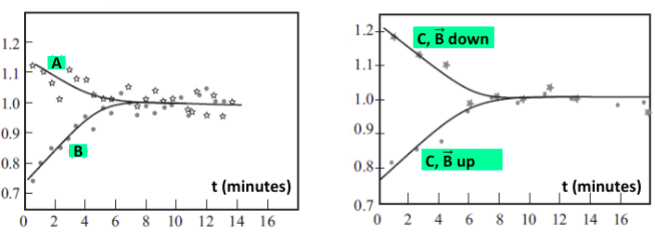
\includegraphics[width=0.6\textwidth]{immagini/fig_plot_wu.png}
        \caption{In A vediamo i due fotoni se sono perpendicolari a $\va{B}$; in B se sono paralleli o antiparalleli; in C vediamo gli elettroni se sono paralleli (o antiparalleli) a $\va{B}$.}
        %\label{fig:plot_wu}
    \end{figure}
    \item L'asimmetria in $t=t_0$ poi scompare; $A>B$ a causa della polarizzazione iniziale (la si misura per usarla successivamente). $A$ e $B$ non dipendono dalla direzione di $\va{B}$ (l'interazione elettromagnetica conserva la parità).
    \item $C$ dipende dalla direzione $\va{B}$, con un rate uguale a quello della polarizzazione: la parità è violata. 
\end{itemize}
Si può reinterpretare l'esperimento con il fatto che esistono solo particelle sinistre.
\begin{itemize}
    \item La conservazione del momento angolare e la polarizzazione forzano la direzione dello spin degli elettroni.
    \item Se lo spin è parallelo all'impulso abbiamo elicità positiva che è proibita ($\propto 1-\beta_e$) con $\beta\approx0.6$.
    \item Se lo spin è antiparallelo all'impulso abbiamo elicità negativa che è permessa.
    \item Ne concludiamo che la direzione opposta a $\va{B}$ è preferita e che il rate $W$ degli elettroni dipende dal $\cos\vartheta$, l'angolo tra il campo magnetico e la velocità dell'elettrone:
    \begin{equation*}
    W(\cos\vartheta)\propto1-P\beta_e\cos\vartheta
    \end{equation*}
\end{itemize}
\subsubsection{Commento di Feynman}
Immagina di parlare con un marziano, o con qualcuno molto lontano, tramite telefono. Non ci è permesso inviargli alcun campione concreto da esaminare; per esempio, se potessimo inviare luce, potremmo mandargli luce polarizzata circolarmente destrorsa. [...] Ma non possiamo dargli niente, possiamo solo parlargli.  
[Feynman spiega come comunicare: matematica, fisica classica, chimica e biologia sono semplici.]  
[...] "Ora metti il cuore sul lato sinistro." Lui dice: "Ehm... il lato sinistro?" [...] Possiamo spiegare a un marziano dove mettere il cuore dicendo: "Ascolta, costruisci un magnete, [... ripeti l'esperimento di Wu ...]; poi, la direzione in cui la corrente scorre attraverso le bobine è quella che noi chiamiamo destra."  
[...] Tuttavia, la materia destrorsa si comporta allo stesso modo dell'antimateria destrorsa? O la materia destrorsa si comporta come l'antimateria sinistrorsa? Gli esperimenti sul decadimento beta, usando il decadimento del positrone invece di quello dell'elettrone, indicano che questa è l'interconnessione: la materia destrorsa funziona nello stesso modo dell'antimateria sinistrorsa.  
[...] Formuliamo una nuova regola che dice che la materia destrorsa è simmetrica all'antimateria sinistrorsa. \\ 
Quindi, se il nostro marziano è fatto di antimateria e gli diamo istruzioni per costruire questo modello destrorso come noi, ovviamente il risultato sarà invertito. Cosa accadrebbe se, dopo molte conversazioni avanti e indietro, insegnassimo l'uno all'altro a costruire astronavi e ci incontrassimo a metà strada nello spazio vuoto? [...]  
Beh, se lui tende la sua mano sinistra... attenzione!  \\
Dalle "\textit{Lectures on Physics}" di Feynman, Volume 1, Capitolo 52: "\textit{Symmetry in Physical Laws}".\\ 

Osservazioni:
- La simmetria di cui parla è "CP" e NON semplicemente "P" o "C".  
- Tuttavia, anche CP è violata (vedi il caso del \(K^0\)).
\subsection{Elicità del neutrino elettronico}
Nel 1958 Goldhaber, Grodzins e Sunyar misurarono l'elicità del neutrino elettronico \(\nu_e\).
\begin{itemize}
    \item Una cruciale conferma della teoria particella-antiparticella sinistra-destra, ma l'elicità di neutrino ed antineutrino non erano ancora state misurate.
    \item L'europio metastabile decade per cattura $K$ in stato eccitato di Samario più un neutrino elettronico, la cui elicità è misurata in questo esperimento.
    \item Il samario eccitato decade nel suo stato fondamentale con emissione di un $\gamma$ ($\gamma_1$ in figura).
    \item Per tale \(\gamma\), la trasmissione nella materia dipende dagli spin degli elettroni; quindi viene applicato un forte campo magnetico (\(\va{B}\)) per polarizzare il ferro.  
    \item I fotoni \(\gamma\) vengono utilizzati per eccitare un altro nucleo di \(\text{Sm}\); solo i fotoni \(\gamma\) della catena precedente possono farlo, producendo un altro \(\gamma\) ($\gamma_2$ in figura).
    \item I fotoni risultanti vengono rivelati.
    \item Alla fine si ottiene 
    \begin{equation*}
    h(\nu_e)=-1.0\pm0.3
    \end{equation*}
    consistente con la teoria particella sinistra e antiparticella destra.
\end{itemize}
\begin{figure}[H]
    \centering
    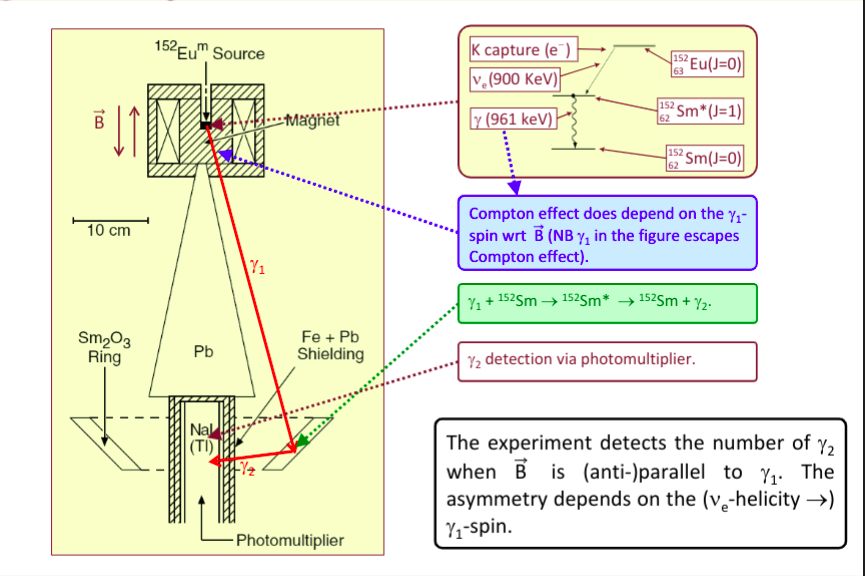
\includegraphics[width=\textwidth]{immagini/fig_exp_nu_hel.png}
\end{figure}
\subsubsection{Da europio a samario a $\gamma$}
\begin{figure}[H]
    \centering
    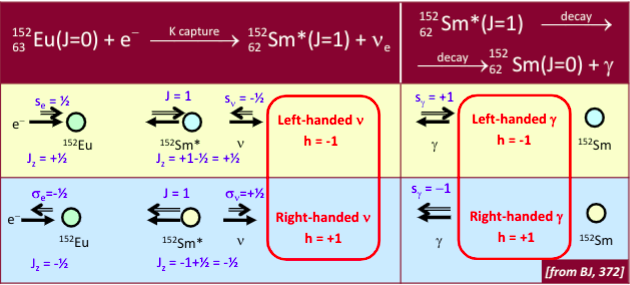
\includegraphics[width=\textwidth]{immagini/fig_schema_eu_sm_gamma.png}
    \caption{}
    \label{fig:schema_eu_sm_gamma}
\end{figure}
\begin{itemize}
    \item Il neutrino è monocromatico con energia di circa 900 keV.
    \item La vita media del samario eccitato è di $10^{-14}$ s, abbastanza breve da trascurre ogni altra interazione.
    \item L'energia di eccitazione del samario è di 961 keV, vicina all'energia del neutrino.
    \item \textit{Solo} per i $\gamma$ nella direzione di rinculo del samario eccitato, la conservazione del momento angolare implica che l'elicità del samario eccitato sia uguale a quella del neutrino che è uguale a quella del $\gamma$ che è $\pm1$ (vedi \autoref{fig:schema_eu_sm_gamma}).
    \item Dunque il metodo consiste in:
    \begin{itemize}
        \item Non puoi misurare direttamente lo spin del neutrino.
        \item Selezioni e misuri i $\gamma$ emessi antiparallelamente al neutrino, cioè nella stessa direzione del samario eccitato
        \item Misuri il loro spin
        \item Ricostruisci l'elicità del neutrino.
    \end{itemize}
\end{itemize}
\subsubsection{Scattering risonante}
\begin{itemize}
    \item Per i fotoni di 961 keV, l'interazione dominante con la materia è l'effetto Compton; la sezione d'urto Compton dipende dallo spin: la trasmissione è maggiore quando lo spin di \(\gamma\) ed \(e^-\) sono paralleli.  
    \item Pertanto, un forte e reversibile campo magnetico (\(\va{B}\)) (ferro saturo) seleziona i \(\gamma\) polarizzati, producendo un'asimmetria tra le due orientazioni di \(\va{B}\).
    \item  È necessario selezionare solo i \(\gamma\) polarizzati in accordo con lo spin del \(\nu_e\), cioè quelli prodotti in direzione opposta al \(\nu_e\). Per fare ciò si utilizza il metodo della diffusione risonante nell'anello di \(Sm_2O_3\) (ossido di samario):  
    \[
    \gamma_1 + {}^{152}\text{Sm} \to {}^{152}\text{Sm}^* \to {}^{152}\text{Sm} + \gamma_2.
    \]  
    \item Un nucleo a riposo, eccitato con un'energia \(E_0\), decade emettendo un \(\gamma\); l'energia del \(\gamma\) nel laboratorio è ridotta di un fattore \(\frac{E_0}{2M}\).
    \item In generale, l'energia di \(\gamma_1\) è degradata e \textbf{non sufficiente} per eccitare il Sm (cioè per produrre \(\gamma_2\)).  
    \item Tuttavia, se \(\gamma_1\) è antiparallelo al \(\nu_e\), il nucleo \({}^{152}\text{Sm}^*\) subisce un rinculo opposto al \(\nu_e\). L'effetto Doppler risultante nella direzione corretta fornisce a \(\gamma_1\) l'energia aggiuntiva necessaria (\(E_\nu \approx E_\gamma\)).  
    \item In conclusione, vengono rivelati solo i \(\gamma\) antiparalleli ai \(\nu_e\), ma questi \(\gamma\) trasportano l'informazione sull'elicità del \(\nu_e\).
\end{itemize}
\subsubsection{Cinematica (conti)}
Consideriamo un decadimento $M\to m+\gamma$ con $E_0=M-m$. Nel riferimento del centro di massa ($M$):
\[
\begin{cases}
    M      &= (M,\;0,\;0,\;0)\\
    \gamma &= (E_\gamma,\;E_\gamma,\;0,\;0)\\
    m      &= (M-E_\gamma,\;-E_\gamma,\;0,\;0)
\end{cases}
\]
\begin{align*}
&m^2=(M-E_\gamma)^2-E_\gamma^2=M^2-2ME_\gamma\implies\\
&\implies E_\gamma=\frac{M^2-m^2}{2M}=\frac{M+m}{2M}E_0=\frac{M+M-E_0}{2M}E_0=E_0\qty(1-\frac{E_0}{2M})
\end{align*}
Ne segue che se il nucleo eccitato $M$ è a riposo, l'energia del fotone nel laboratorio è minore dell'energia di eccitazione $E_0$. Dunque non basta per eccitare un altro nucleo a riposo. Affinché questo avvenga, il nucleo si deve muovere nella direzione giusta e con l'energia appropriata.
\subsection{Decadimento debole: i \texorpdfstring{$\pi$}{π}}
\begin{itemize}
    \item Il \(\pi^\pm\) è l'adrone più leggero, quindi può decadere solo tramite processi deboli carichi semileptonici (\(CC\)), come (considerando solo \(\pi^+\); per \(\pi^-\), applicare \(C\)):  
    \[
    \pi^+ \to \mu^+ \nu_\mu, \quad \pi^+ \to e^+ \nu_e
    \]
    \item In realtà, il decadimento avviene quasi esclusivamente in \(\mu\): il decadimento elettronico è soppresso da un fattore \(\approx 8000\), non comprensibile, anche perché il decadimento \((\pi \to e)\) è favorito dallo spazio delle fasi.  
    \item La ragione risiede nell'elicità:
    \begin{itemize}
        \item nel sistema di riferimento del \(\pi^+\), gli \textit{impulsi} di \(\ell^+\) e \(\nu_\ell\) devono essere \textit{opposti};
        \item poiché il \(\pi^+\) ha \textit{spin} \(0\), gli spin di \(\ell^+\) e \(\nu\) devono essere anch'essi \textit{opposti};
        \item quindi, le due particelle devono avere la \textit{stessa elicità};
        \item poiché il \(\nu\) (una particella quasi priva di massa) deve avere elicità negativa, il \(\ell^+\) (un'antiparticella con massa) è costretto anch'esso ad avere elicità negativa;
        \item di conseguenza, la transizione è soppressa da un fattore \((1 - \beta_\ell)\);
        \item il \(e^+\) è ultrarelativistico (\(p_e \approx m_\pi / 2 \gg m_e\)), mentre il \(\mu^+\) ha un \(\beta\) più piccolo;
        \item quindi, il decadimento \(\pi \to e\) è \textit{fortemente soppresso} rispetto a \(\pi \to \mu\).
    \end{itemize}
\end{itemize}
\subsubsection{Cinematica (conti) più generale}
Decadimento \( M \to a + b \). Calcola \( p = |\vec{p}_a| = |\vec{p}_b| \) nel riferimento del centro di massa ($M$):  

\[
\text{CM:} \quad
\begin{cases}
(M, 0, 0, 0) \\
\left(\sqrt{m_a^2 + p^2}, p, 0, 0 \right) \\
\left(\sqrt{m_b^2 + p^2}, -p, 0, 0 \right)
\end{cases}
\]
Da conservazione di energia  abbiamo 
\[
M = \sqrt{m_a^2 + p^2} + \sqrt{m_b^2 + p^2};
\]

\[
2 \sqrt{m_a^2 + p^2} \sqrt{m_b^2 + p^2} = M^2 - m_a^2 - m_b^2 - 2p^2;
\]

\[
4 \left[ m_a^2 m_b^2 + p^2 \left( m_a^2 + m_b^2 \right) + p^4 \right] 
= \left( M^2 - m_a^2 - m_b^2 \right)^2 + 4 p^4 - 4p^2 \left( M^2 - m_a^2 - m_b^2 \right);
\]

\[
4p^2 \left[ \left( m_a^2 + m_b^2 \right) + \left( M^2 - m_a^2 - m_b^2 \right) \right] 
= -4m_a^2 m_b^2 + \left( M^2 - m_a^2 - m_b^2 \right)^2;
\]

\[
4p^2 M^2 = \left( M^2 - m_a^2 - m_b^2 \right)^2 - 2m_a^2 m_b^2 
\implies
\]

\[
p^2 = \frac{\left[ M^2 - (m_a - m_b)^2 \right] \left[ M^2 - (m_a + m_b)^2 \right]}{4M^2}.
\]

\begin{enumerate}
    \item[\textbf{a)}] \( m_a = m_b = m \):  
    \[
    p^2 = \frac{M^2 - 4m^2}{4}, \quad p = \frac{(M + 2m)(M - 2m)}{4};
    \]  
    e.g. \( K^0 \to \pi^0 \pi^0 \).

    \item[\textbf{b)}] \( m_a=m_b = 0 \):  
    \[
    p^2 = \frac{M^2}{4}, \quad p = \frac{M}{2};
    \]  
    e.g. \( \pi^0 \to \gamma \gamma, \; H \to \gamma \gamma \).

    \item[\textbf{c)}] \( m_a = m, \; m_b = 0 \):  
    \[
    p = \frac{M^2 - m^2}{2M} = \frac{M}{2} \left[ 1 - \left( \frac{m}{M} \right)^2 \right];
    \]  
    e.g. \( \pi^+ \to \mu^+ \nu_\mu, \; W^* \to W \gamma \).
\end{enumerate}
\subsubsection{Decadimento $\pi^\pm\to e^\pm/\mu^\pm$}
Calcoliamo il fattore nel decadimento dei pioni tra elettroni e muoni.\\
Consideriamo le seguenti variabili per il decadimento $\pi\to\ell$:
\begin{itemize}
    \item $p$ = impulso del prodotto di decadimento;
    \item $p_\ell=\dv{N}{E\_{tot}}$ = fattore spazio delle fasi;
    \item $\dd{N}=\frac{1}{(2\pi)^3}Vp^2\dd{p}\dd{\Omega}$;
    \item $1-\beta_\ell$ = soppressione di elicità;
    \item $BR_\ell = \frac{\Gamma_\ell}{\Gamma\_{tot}} \propto \rho_\ell\times(1-\beta_\ell)$.
\end{itemize}
In qesto caso il decadimento è isotropo, quindi
\begin{equation*}
    \rho_\ell \propto p^2\dv{p}{E\_{tot}}
\end{equation*}
Da conservazione del quadrimpulso (usa sottosezione precedente)
\begin{align*}
&p_\ell=p_\nu=E_\nu=p;\qq{}E\_{tot}=m_\pi;\qq{}E_\ell=m_\pi-E_\nu=m_\pi-p\\
&p=\qty(\frac{m_\pi^2-m_\ell^2}{2m_\pi})^2=\frac{E\_{tot}}{2}-\frac{m_\ell^2}{2E\_{tot}}\;\;\dv{p}{E\_{tot}}=\frac{1}{2}+\frac{m_\ell^2}{2m_\pi^2}=\frac{m_\pi^2+m_\ell^2}{2m_\pi^2};\\
&p_\ell\propto\qty(\frac{m_\pi^2-m_\ell^2}{2m_\pi})^2\frac{m_\pi^2+m_\ell^2}{2m_\pi^2}=\frac{(m_\pi^2+m_\ell^2)(m_\pi^2-m_\ell^2)^2}{8m_\pi^4}
\end{align*}
Il termine al denominatore $8m_\pi^4$ è irrilevante, invece sappiamo che $\rho_e>\rho_\mu$.\\
\begin{equation*}
1-\beta_\ell=1-\frac{p_\ell}{E_\ell}=1-\frac{p}{m_\pi-p}=\dots=\frac{2m_\ell^2}{m_\pi^2+m_\ell^2}\implies 1-\beta_e\lll1-\beta_\mu
\end{equation*}
\begin{equation*}
    BR_\ell\propto(m_\pi^2+m_\ell^2)(m_\pi^2-m_\ell^2)^2\frac{2m_\ell^2}{m_\pi^2+m_\ell^2}\propto m_\ell^2(m_\pi^2-m_\ell^2)^2
\end{equation*}
Per gli elettroni, visto che $m_e\ll m_\pi$, abbiamo:
\begin{equation*}
    \frac{\textnormal{BR}(\pi^+\to e^+\nu_e)}{\textnormal{BR}(\pi^+\to \mu^+\nu_\mu)}=\qty(\frac{m_e}{m_\mu}\frac{m_\pi^2-m_e^2}{m_\pi^2-m_\mu^2})^2\approx1.28\times10^{-4}
\end{equation*}
Sperimentalmente si misura:
\begin{equation*}
    \frac{\textnormal{BR}(\pi^+\to e^+\nu_e)}{\textnormal{BR}(\pi^+\to \mu^+\nu_\mu)}=1.23\times10^{-4}
\end{equation*}